\chapter{Initial exploration}
\label{cha:1}
In this chapter an initial exploration of the problem is done. The backpropagation algorithm is compared relative to the simultaneous approach for a couple small regression problems.

For the backpropagation algorithm the experiments were done using the Neural Network Toolbox in MATLAB version 2018a. The training was done using the \texttt{trainlm} procedure which implements a Levenberg-Marquardt backpropagation algorithm. GRADIENT DESCENT

For the simultaneous approach the problems were set up using the YALMIP version R20190425 optimization library, implementing the OCP detailed in equation \ref{ocp-eq}. This problem was then solved using MATLAB's \texttt{fmincon} procedure.



\section{First experiment}
The first experiment conducted was to apply both algorithms to a test problem. A small neural network is constructed with 2 hidden layers with each layer containing 3 nodes with tansig activation function. The activation function was chosen because it works well for a small network. This network is then trained to approximate a piece of a sine function. Both algorithms are trained for 100 epochs. Figure \ref{} shows the training performance for a training run of each algorithm. Both perform well, but the simultaneous approach is much slower. This can be due to the fact that the new algorithm is not well optimized.

\begin{figure}
     \centering
     \begin{subfigure}[b]{0.8\textwidth}
         \centering
         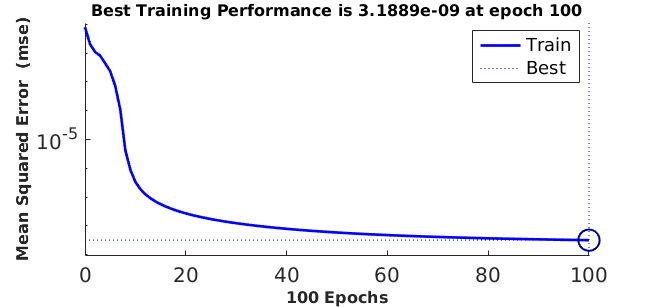
\includegraphics[width=\textwidth]{back_test_1}
         \caption{Training performance of backpropagation}
         \label{fig:y equals x}
     \end{subfigure}
     \begin{subfigure}[b]{0.8\textwidth}
         \centering
         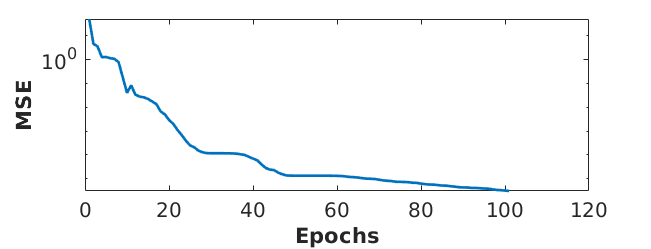
\includegraphics[width=\textwidth]{back_test_12}
         \caption{Training performance of simultaneous approach}
     \end{subfigure}
     \begin{subfigure}[b]{0.8\textwidth}
         \centering
         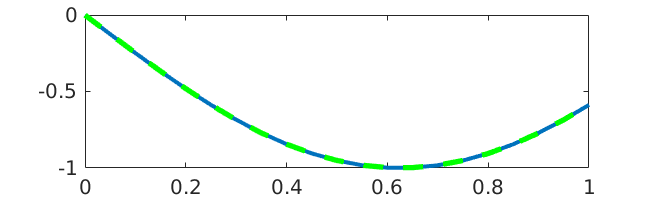
\includegraphics[width=\textwidth]{sine}
         \caption{Sine function}
     \end{subfigure}
        \caption{Performance of algorithms for simple regression problem}
        \label{fig:three graphs}
\end{figure}




The backpropagation algorithm converges every time for this problem, taking anywhere between 10 and 1000 iterations. The stopping criteria is that the validation error increases for 6 consecutive iterations.

The simultaneous approach also converges if the intial conditions are set correctly. The weight variables are randomly initialized and the state variables are initialized by simulating the network once using the input vector, ensuring the initial point is feasible. The method converges every time, but it runs much slower. Its not known if this is due to the difference in optimization of the algorithms and the fact that the backpropagation algorithm is running on my GPU instead of the CPU.

\section{Second experiment}
For this experiment again the same regression problem of the previous section is considered but with a different network. Here a network of two layers is used, with 8 neurons in each layer, but using a ReLU activation function. 

The backpropagation function will almost always converge for this problem.

For the simultaneous approach the RELU activation function will have to be reformulated, in order to have smooth constraints. The ReLU function can be transformed as follows:

   \begin{gather*}
   x_{k+1}^j = \max(W_kx_k^j,0) \\
   \Updownarrow \\
   x_{k+1}^j = -\min(-W_kx_k^j,0) \\
   \Updownarrow \\
   \min(x_{k+1}^j-W_kx_k^j) = 0 \\
   \Updownarrow \\
   (x_{k+1}^j-W_kx_k^j)^\top x_{k+1}^j = 0,\\
   x_{k+1}^j\geq 0,x_{k+1}^j-W_kx_k^j\geq 0
   \end{gather*}
   
But even using these smooth constraints, the algorithm will usually not converge. It might be that this is due to the use of the fmincon optimization method, which is very general. In the next chapter the simultaneous approach will be rewritten in python using a more specific algorithm.

\section{Further exploration}
There are many options that can be explored to further compare these algorithms.

\begin{itemize}
\item Activation function: ReLU is the most popular activation function in the field. Others are tansig, sigmoid, SoftPlus, leaky ReLU, etc.
\item Network size: Networks can be up to thousands of neurons wide and hundreds of layers deep. 
\item Network architecture: There is a huge variety of possible network architectures. Convolutional neural networks for example are very popular for image recognition.
\item Test problems: Neural networks have many applications. Some applications could benefit more from this training method than others.
\item Optimization algorithm: fmincon is quite a general method, a more specific method might perform better
\item Stopping criteria and initial conditions

These will be explored in the next chapters

\end{itemize}

The option that will be explored in the next chapter, will be changing the optimization algorithm. The \texttt{fmincon} method will be replaced by a specifically written algorithm, exploiting the structure of the problem.





%%% Local Variables: 
%%% mode: latex
%%% TeX-master: "thesis"
%%% End: 
